\documentclass[10pt]{article}
\usepackage{graphicx}
\graphicspath{ {images/} }
\usepackage{amsmath}
\begin{document}

\title{Homework 5 - Functions}
\author{Michael Gould\\ 
CS 506 - Online Foundations of CS}

\maketitle
1. Consider the following sets of ordered pairs.\\

(a) $S_1 = \{(1,a),(2,b),(3,c),(4,d)\}$

(b) $S_2 = \{(1,a),(2,b),(3,d),(4,d)\}$

(c) $S_3 = \{(1,a),(1,b),(2,c),(2,d)\}$\\

Determine if each set defines a \textit{function} from $X = {1,2,3,4}$ to $Y = {a,b,c,d}$.  If the set is a function, then:\\

Determine its domain $D$, co-domain $Y$ and range $R$.

Is the function one-to-one?

Is the function \textit{onto}

If the function is one-to-one and onto, find its inverse.\\

1(a).  Describes a function where the domain $D = \{1,2,3,4\}$, the co-domain $Y = \{a,b,c,d\}$, and the range $R = \{a,b,c,d\}$.  The function is in fact one-to-one, because no two values in the domain map to the same value in the range.  The function can be described as being \textit{onto}, because both the range as well as the co-domain are equivalent($R = Y$).  Given that the function is both one-to-one as well as onto, we can find the inverse, expressed as follows in ordered pairs:

$$f^{-1} = \{(a,1),(b,2),(c,3),(d,4)\}$$

1(b).  Describes a function where the domain $D = \{1,2,3,4\}$, the co-domain $Y = \{a,b,c,d\}$, and the range $R = \{a,b,d\}$.  The function is many-to-one, given that two values from the domain map to a same value in the range (specifically $f(3)$ and $f(4)$ which both map to $d$).  The function can be described as being into, because the co-domain is a proper sub-set of the range ($R \subset Y$), meaning that all values of the range can be found in the co-domain but not all values in the co-domain are represented in the range.  Because this function is many-to-one, there is no inverse.

1(c). Does not describe a function, it does not define $f(3)$ or $f(4)$, as well as neither $f(1)$ nor $f(2)$ being unique. (That is, $f(1,a) \in f$ and $f(1,b) \in f$)


2. The functions $f(n) = n^2$ and $g(n) = 2n$ are defined on the set of positive real numbers.\\

(a) Find the composition of $f \circ g$. (The composition $(f \circ g)(n)$ is defined as $f(g(n)).$)

(b) Find the composition $g \circ f$

(c) Find the inverse functions $f^{-1}$ and $g^{-1}$.\\

2(a).$$(f \circ g)(n) = f(g(n)) = (2n)^2 = 4n^2$$

2(b).$$(g \circ f)(n) = g(f(n)) = 2(x^2) = 2x^2$$

2(c).$$f^{-1}(x) = \sqrt{x}$$  
$$g^{-1}(x) =  \frac{x}{2}$$

3. A sequence $(F1,F2,F3,...)$ is defined recursively as follows. (this recursive definition is called a \textit{recurrance equation}.)

\begin{equation}
  f(x)=\begin{cases}
    1, & $n = 1$\\
    2F_{n-1} + 1, & $c $\geq$ 2$\\
  \end{cases}
\end{equation}

(a) Compute $F_1,F_2,...F_10$ and tabulate results.

(b) Prove by induction on $n$ that
$$F_n = 2^n - 1, n \geq 1.$$

3(a).

\center
\begin{tabular}{@{ }c@{ }@{ }|c c@{ }@{ }c@{ }@{ }c@{ }@{ }c@{ }@c}
$f(x)$ & Output \\
\hline
$F1$ & 1 & & & \\
$F2$ & 2(1) + 1 = 3 & \\
$F3$ & 2(3) + 1 = 7 & & & \\
$F4$ & 2(7) + 1 = 15& & & \\
$F5$ & 2(15) + 1 = 31& & & \\
$F6$ & 2(31) + 1 = 63& & & \\
$F7$ & 2(63) + 1 = 127& & & \\
$F8$ & 2(127) + 1 = 255& & & \\
$F9$ & 2(255) + 1 = 511& & & \\
$F10$ & 2(511) + 1 = 1023& & & \\
\end{tabular}
\flushleft

3(b). Provided the hypothesis $P(n): F_n = 2^n-1 \forall n \geq 1$, to use simple induction, we must begin by proving a base case.  In this instance I have chosen the case of $n=1$, which as shown here
$$F_1 = 2^1 - 1 \Rightarrow 1 \geq 1$$
proves to be true.  We are now to assume that $P(1) \wedge P(2) \wedge ... \wedge P(k-1)$ for some integer $k$, which we will use to prove $P(k)$.  We assume, given our base case, that the following is also true:
$$P(k-1): F_{k-1} = 2^{k-1} - 1$$
$$P(k): F_k = 2^k - 1$$
Using the following substitutions and algebra we can show through induction that:
$$F_k = 2F_{k-1} + 1$$
$$\Rightarrow 2(2^{k-1} - 1) + 1$$
$$\Rightarrow 2^k - 2 + 1$$
$$\Rightarrow 2^k -1$$

4. the Fibonacci sequence is defined recursively as follows:

\begin{equation}
  f(x)=\begin{cases}
    1, & $n = 1$\\
    2, & $n = 2$\\
    F_{n-1} + F_{n-2}, & $n $\geq$ 3$\\
  \end{cases}
\end{equation}

(a) Compute and tabulate $F_1,F_2,...F_12$.

(b) Prove by induction that for all $n \geq 1$,
$$F_n \leq (1.62)^{n-1}$$

(c) Prove by induction that for all $n \geq 1$,
$$F_n \geq (1.61)^{n-2}$$

4(a).

\center
\begin{tabular}{@{ }c@{ }@{ }|c c@{ }@{ }c@{ }@{ }c@{ }@{ }c@{ }@c}
$f(x)$ & Output \\
\hline
$F1$ & 1 & & & \\
$F2$ & 2 & & & \\
$F3$ & 2 + 1 = 3 & & & \\
$F4$ & 3 + 2 = 5 & & & \\
$F5$ & 5 + 3 = 8 & & & \\
$F7$ & 8 + 5 = 13 & & & \\
$F8$ & 13 + 8 = 21 & & & \\
$F9$ & 21 + 13 = 34 & & & \\
$F10$ & 34 + 21 = 55 & & & \\
$F11$ & 55 + 34 = 89 & & & \\
$F12$ & 89 + 55 = 144 & & & \\
\end{tabular}
\flushleft

4(b). Provided the hypothesis $P(n): F_n \leq (1.62)^{n-1}$ $\forall n \geq 1$ to use the necessary strong induction, we must begin by providing some base cases.  For these instances I have chosen the values $n=1$ as well as $n=2$
$$P(1): F_1 \leq (1.62)^0 \Rightarrow 1 \leq 1$$
$$P(2): F_2 \leq (1.62)^1 \Rightarrow 1 \leq 1.62$$

which proves to be true.  We are now to assume that $P(1) \wedge P(2) \wedge ... \wedge P(k-1)$ for some integer $k$, which we will use to prove $P(k)$.  We assume, given our base cases and other information, that the following is also true:
$$P(k-2): F_{k-2} \leq (1.62)^{k-3}$$
$$P(k-1): F_{k-1} \leq (1.62)^{k-2}$$
$$P(k): F_k \leq (1.62)^{k-1}$$

Now, with substitutions, information from the recurrance equation, and some inequality properties, we can manipulate the equations as follows:

$$F_k = F_{k-1} + F_{k-2} \leq F_{k-1} + (1.62)^{k-3}$$
$$F_k = F_{k-1} + F_{k-2} \leq (1.62)^{k-2} + (1.62)^{k-3}$$
$$\Rightarrow F_k \leq (1.62)^{k-2} + (1.62)^{k-3}$$
$$\Rightarrow F_k \leq (1.62)^{k-3}[1.62 + 1]$$
$$\Rightarrow F_k \leq (1.62)^{k-3}[2.62]\stackrel{?}{\leq}(1.62)^{k-3}(1.62)^2$$

$$(1.62)^2 = 2.6244 \geq 2.62)$$
$$\Rightarrow F_k \leq (1.62)^{k-3}(1.62)^2$$
$$\Rightarrow F_k \leq (1.62)^{k-1}$$

4(c).Provided the hypothesis $P(n): F_n \geq (1.61)^{n-2}$ $\forall n \geq 1$ to use the necessary strong induction, we must begin by providing some base cases.  For these instances I have chosen the values $n=2$ as well as $n=3$

$$P(1): F_1 \geq (1.61)^{1-2} \Rightarrow 1 \geq \frac{1}{1.61}$$
$$P(2): F_2 \geq (1.61)^{2-2} \Rightarrow 1 \geq 1$$

which prove to be true.  We now assume that $P(1) \wedge P(2) \wedge ... \wedge P(k-1)$ for some integer $k$, which we will use to prove $P(k)$.  We assume given our base cases and other information that the following is true:

$$P(k-2): F_{k-2} \geq (1.61)^{k-4}$$
$$P(k-1): F_{k-1} \geq (1.61)^{k-3}$$
$$P(k): F_k \geq (1.61)^{k-2}$$

Now, with substitutions, information from the recurrance equation, and some inequality properties, we can manipulate the equations as follows:

$$F_k = F_{k-1} + F_{k-2} \geq F_{k-1} + (1.61)^{k-4}$$
$$F_k = F_{k-1} + F_{k-2} \geq (1.61)^{k-3} + (1.61)^{k-4}$$ 
$$\Rightarrow F_k \geq (1.61)^{k-3} + (1.61)^{k-4}$$
$$\Rightarrow F_k \geq (1.61)^{k-4}[1.61 + 1]$$
$$\Rightarrow F_k \geq (1.61)^{k-4}[2.61]\stackrel{?}{\geq}(1.61)^{k-4}(1.61)^2$$

$$(1.61)^2 = 2.5921 \leq 2.61$$
$$\Rightarrow F_k \geq (1.61)^{k-4}(1.61)^2$$
$$\Rightarrow F_k \leq (1.61)^{k-2}$$

5. Let ${F_n}$ be the Fibonacci sequence (defined above).  Prove by induction that for all $n \geq 1$,
$$S(n): \sum\limits_{k=1}^n F_k = F_{n+2} - 1$$

Provided the hypothesis$S(n): \sum\limits_{k=1}^n F_k = F_{n+2} - 1$ to use induction, we must first prove the base case.  For this instance, I have chosen the value $n=1$

$$S(1): \sum\limits_{k=1}^1 F_k = 1 = F_{n+2} - 1 = F_{1+2} - 1 = F_3 - 1 = 2 - 1 = 1$$

Thus the base case holds true for the hypothesis.  We now assume that $S(1) \wedge S(2) \wedge ... \wedge S(n-1)$ for some integer $n$, which we will use to prove $S(n)$.  We assume given our base cases and other information that the following is true:

$$S(n): \sum\limits_{k=1}^n F_k = F_1 + F_2 + ... + F_n = F_{n+2} - 1$$
$$S(n+1): \sum\limits_{k=1}^{n+1} F_k = F_1 + F_2 + ... + F_n + F_{n+1} = F_{(n+1)+2} - 1$$

Now, with substitutions and information from the recurrance equation, we can manipulate the equations as follows:

$$S(n+1): \sum\limits_{k=1}^{n+1} F_k = F_1 + F_2 + ... + F_n + F_{n+1} = F_{(n+1)+2} - 1$$
$$S(n+1): \sum\limits_{k=1}^n F_k + F_{n+1} = F_{n+3} - 1$$
$$S(n+1): \sum\limits_{k=1}^n F_k = F_{n+2} - 1$$

6. Consider the following relations.\\

(a) $R_1 = \{(1,1),(1,2),(2,1),(2,2),(3,3)\}$

(b) $R_2 = $\{$(x,y)|x,y$ are positive integers$ \leq$ 3, and $x+y \leq 5$\}

(c) $R_3 = $\{$(x,y)|x,y$ are positive integers$ \leq$ 3, and $x\leq y \leq x + 2$\}

For each relation,\\

Show the relation as a \textit{set of ordered pairs} (if not in that form already), in \textit{table} form, and in the form of a \textit{directed graph}. (Show the graph with two columns of vertices, where the domain is the left column and the range is the right column.)

Determine whether the relation is \textit{reflexive, symmetric, antisymmetric, transitive.} (Justify your answers.)

Determine if the relation is a \textit{partial order} or an \textit{equivalence relation}.  If the latter is true, then specify the equivalence  classes.\\

6(a). The relation comes to us in the form of ordered pairs. In the form of a table, it is as follows:
\center
\begin{tabular}{@{ }c@{ }@{ }|c c@{ }@{ }c@{ }@{ }c@{ }@{ }c@{ }@c}
\hline
1 & 1 \\
1 & 2 \\
2 & 1 \\
2 & 2 \\
3 & 3 \\
\end{tabular}
\flushleft

As a graph it looks as follows:

\center
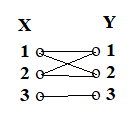
\includegraphics{6a}
\flushleft

\textbf{Reflexive:} Given that the function is on the domain of $X = \{1,2,3\}$The above relation is reflexive, because for every $X$ there exsits the ordered pair $(x,x)$.

\textbf{Symmetric:} The above relation is in fact symmetric, because for all values of $x$ and $y$ there exsists $(x,y)$ as well as a cooresponding $(y,x)$ in the same relation.

\textbf{Anti-Symmetric:} As explained above, because of the symmetric properties of the relation, it is impossible to be anti-symmetric, for no relation can have both properties at the same time.

\textbf{Transitive:} The above relation is in fact transitive, because for every $(x,y)$ and $(y,z)$ there exsists $(x,z)$

Given the nature of the relation (that it is \textbf{Reflexive},\textbf{Symmetric}, and \textbf{Transitive}) this means that it is an \textit{equivalence relation}.  Its equivalence classes are as follows:

\center
Block 1: \{1,2\}\\
Block 2: \{1,2\}\\
Block 3: \{3\}\\
\flushleft

6(b). The relation in as a set of ordered pairs looks as follows:
$$R_2 = \{(1,1),(1,2),(1,3),(2,1),(2,2),(2,3),(3,1),(3,2)\}$$

As a table the relation looks as follows:
\center
\begin{tabular}{@{ }c@{ }@{ }|c c@{ }@{ }c@{ }@{ }c@{ }@{ }c@{ }@c}
\hline
1 & 1 \\
1 & 2 \\
1 & 3 \\
2 & 1 \\
2 & 2 \\
2 & 3 \\
3 & 1 \\
3 & 2 \\
\end{tabular}
\flushleft

\textbf{Reflexive:} The above relation is not reflexive, due to the fact that on the set of $\{1,2,3\}$ there exists no relationship $(3,3)$

\textbf{Symmetric:} The above relation is in fact Symmetric because each relationship $(x,y)$ has within the same relation a cooresponding relationship $(y,x)$

\textbf{Anti-Symmetric:} By definition, because the relation is symmetric, this relation cannot also be anti-symmetric

\textbf{Transitive:} This relation is not transitive, this is due to that there exists an $x,y,z$ that does not fulfill the transitive definition, specifically in this relation $(3,1) \in R, (1,3) \in R, (3,3) \notin R$ 

Due to the fact that the relation is not reflexive, it cannot be an equivalence relation or a partial order.

As a graph it looks as follows:

\center
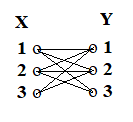
\includegraphics{6b}
\flushleft

6(c).The relation in a set of ordered pairs looks as follows:
$$R_3 = \{(1,1),(1,2),(1,3),(2,2),(2,3),(3,3)\}$$

As a table the relation looks as follows:
\center
\begin{tabular}{@{ }c@{ }@{ }|c c@{ }@{ }c@{ }@{ }c@{ }@{ }c@{ }@c}
\hline
1 & 1 \\
1 & 2 \\
1 & 3 \\
2 & 2 \\
2 & 3 \\
3 & 3 \\
\end{tabular}
\flushleft

As a graph it looks as follows:

\center
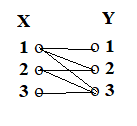
\includegraphics{6c}
\flushleft

\textbf{Reflexive:} This relation is in fact transitive, because on the set of $X$ where $x\leq3$ there exsist all instances of $(x,x)$

\textbf{Symmetric:} This relation is not symmetric, due to the fact that there exists a $(x,y)$ for which there is no cooresponding $(y,x)$, in this relation speficically: $(1,2) \in R$ and $(2,1) \notin R$

\textbf{Anti-Symmetric:} This relation is in fact anti-symmetric, thanks to the fact that for all $(x,y)$ there exist no instance of $(y,x)$

\textbf{Transitive:} This relation is also Transitive, because for each and every $x,y,z \in R$ there exist $(x,y) \in R$, $(y,z) \in R$, and $(x,z) \in R$  

In addition to being \textbf{Reflexive},\textbf{Anti-Symmetric}, and \textbf{Transitive}, this list is also a partial order, because the pairs of integers are not related.  An example of such an instance would be (2,1), because it does not fulfill the definition of $x \leq y$ and therefore is not a part of the relation.\\

7. For each of the following relations show the Boolean matrix $A$ and compute the Boolean matrix $A^2$.  Then, by comparing $A$ and $A^2$, determine whether the relation is transitive, and justify your answer.\\

(a) $R_1 = \{(1,1),(1,3),(2,2),(3,1),(3,3)\}$

(b) $R_2 = \{(1,1),(2,1),(2,3),(3,1)\}$

(c) $R_3 = \{(1,1),(2,3),(3,1)\}$\\

To test for transitivity, we need just compare the initial matrix $A$ with that of the $A^2$.  Using substitution of the definition of transitivity, as well as the construction of Boolean matrices, transitivity can be defined as being having the following quality: $\forall Ai$  $\forall Aj$, if $A^2[i,j]$  then $A[i,j] = 1$.  we simply administer this same test to the following matrices and can quickly find their transitivity or lack thereof.

7(a).
$$A = 
\begin{bmatrix}
1 & 0 & 1 \\
0 & 1 & 0 \\
1 & 0 & 1 \\
\end{bmatrix}
A^2 = 
\begin{bmatrix}
1 & 0 & 1 \\
0 & 1 & 0 \\
1 & 0 & 1 \\
\end{bmatrix}
$$
Transitive (see above explanation)

7(b).
$$A = 
\begin{bmatrix}
1 & 0 & 0 \\
1 & 0 & 1 \\
1 & 0 & 0 \\
\end{bmatrix}
A^2 = 
\begin{bmatrix}
1 & 0 & 0 \\
1 & 0 & 0 \\
1 & 0 & 0 \\
\end{bmatrix}
$$
Not-transitive $(A[2,3] \neq A^2[2,3]$

7(c).
$$A = 
\begin{bmatrix}
1 & 0 & 0 \\
0 & 0 & 1 \\
1 & 0 & 0 \\
\end{bmatrix}
A^2 = 
\begin{bmatrix}
1 & 0 & 0 \\
1 & 0 & 0 \\
1 & 0 & 0 \\
\end{bmatrix}
$$
Not-transitive $(A[2,3] \neq A^2[2,3]$ AND $(A[2,1] \neq A^2[2,1]$

\end{document}